\documentclass[../pbr.tex]{subfile}

\begin{document}
\section{Light Transport I}%
\label{sec:light_transport_i}

The primary premise of a physically based render is the simulate the travel of
light throughout the scene and its interactions with the objects and materials
present. Conceptually consider rays of light leaving a light in a room. As the
light bounces around the room it at some point either hits the observers eye,
or it bounces away. This basic description is shown in Figure
\ref{fig:p1_light_transport}.

\begin{figure}[htpb]
\begin{center}
\begin{tikzpicture}[scale=1, transform shape]
  \draw (0,0) -- (5,0) -- (5,5) -- (0,5) -- (0,0);
  \draw (4,1) circle (1);
  \node at (1,1){\faEye};
  \node at (2.5, 4){\faSunO};
  \draw[->](2.7,4.0) -- (5.0,4.0);
  \draw[->](5.0,4.0) -- (1.2,1.1);
  \draw[->](2.6,3.8) -- (3.5,1.9);
  \draw[->](3.5,1.9) -- (0.1,4.8);
\end{tikzpicture}
\end{center}
\caption{Rays of light propagating from a light source to an observer}%
\label{fig:p1_light_transport}
\end{figure}

From this image it becomes clear that one would need to simulate billions of
rays of light for any semblance of an image to form. This is because the
observer can be considered a single point in space, then the probability that a
ray will travel through an infinitesimal point in the entirety of the region is
for all intensive purposes zero. So with this method, we would need to simulate
an infinite number of light sources before enough light reaches the observer to
construct a representation of the scene.

The way to solve this issue, is to follow the light backwards. The
transport of light, in this macroscopic domain, is deterministic, and perfectly
reversible. That is to say that if there is an incident ray in direction
$\vec{a}$, and it reflects in direction $\vec{b}$, then a light incoming from
direction $-\vec{b}$ will be reflected in direction $-\vec{a}$.

The method that rendering systems actually use is to trace the rays of light
from the observer into the scene, and then wait until the rays hit a light
source. Since the light sources are not point objects, but have a surface, then
the probability that a ray will hit a light source could still be small, but it
is significantly more probable than a ray hitting the observer. Taking a look
at the same scene as before, with this new method is shown in Figure
\ref{fig:p1_observer_light_transport}.

\begin{figure}[htpb]
\begin{center}
\begin{tikzpicture}[scale=1, transform shape]
  \draw (0,0) -- (5,0) -- (5,5) -- (0,5) -- (0,0);
  \draw (4,1) circle (1);
  \node at (1,1){\faEye};
  \node at (2.5, 4){\faSunO};
  \draw[<-](2.7,4.0) -- (5.0,4.0);
  \draw[<-](5.0,4.0) -- (1.2,1.1);
  \draw[->](1.3,1.0) -- (3.1,1.4);
  \draw[->](3.1,1.4) -- (2.6,3.8);
  \draw[->](1.2,0.9) -- (2.5,0.0);
  \draw[->](2.5,0.0) -- (3.2,0.4);
\end{tikzpicture}
\end{center}
\caption{Rays of light propagating from an observer to a light source}%
\label{fig:p1_observer_light_transport}
\end{figure}

It is clear that even though not all rays will result in hitting a light
source, a significantly larger number will travel between a light source and
the observer. Because of this improvement this is the method that we will use
for tracing rays of light throughout the scene.

\end{document}
